\documentclass{cumcmthesis}
% \documentclass[withoutpreface,bwprint]{cumcmthesis} %去掉封面与编号页,电子版提交的时候使用。

\usepackage{subcaption} % 子标题
\title{葡萄酒的分级策略}
\tihao{C}
\baominghao{0001}
\schoolname{上海对外经贸大学}
\membera{华光辉 }
\memberb{许炜 }
\memberc{朱墨 }
\supervisor{待定 }
\yearinput{2021}
\monthinput{09}
\dayinput{10}


\RequirePackage{booktabs,tabularx,multirow,longtable,makecell,array}
\newcolumntype{Y}{>{\centering\arraybackslash}X}
\RequirePackage{graphicx}

\usepackage{float} %设置图片浮动位置的宏包


\begin{document}
	 \maketitle
	\begin{abstract}
		这是摘要,本文通过主成分分析法通过对葡萄酒理化指标的分析将相关性较强的提取为一个主成分,对主成分的贡献率进行排序,最终得到葡萄的得分,以此作为分级的依据。
		
		
		
		\vspace*{2\baselineskip}   %空白间距
		要求摘要单独占据一页 
		
		\keywords{评价策略{}\quad  主成分分析法\quad   假设检验\quad  理化指标}
	\end{abstract}

	\section{问题重述}
	\subsection{问题背景}
	葡萄酒
	\subsection{问题提出}
	如何对葡萄酒进行科学评价
	
	\section{模型假设}
	提出假设
	\begin{assumption}
		葡萄酒品质只和这些因素有关
		\label{asu:jiashe1}
	\end{assumption}
\par
对\cref{asu:jiashe1}进行说明

	\begin{assumption}
	葡萄酒品质只和这些因素有关
	\label{asu:jiashe2}
	\end{assumption}
\par
	在这里引用\cref{asu:jiashe1}
	
	
	\section{符号说明}
	
	\begin{center}
		\begin{tabularx}{0.7\textwidth}{c@{\hspace{1pc}}|@{\hspace{2pc}}X}
			\Xhline{0.08em}
			符号 & \multicolumn{1}{c}{符号说明}\\
			\Xhline{0.05em}
			$\delta$ & 赤纬角\\
			$\beta$ & 经度\\
			$\alpha$ & 纬度\\
			$r$ & 地球半径\\
			$\gamma$ & 太阳光与杆所成的夹角\\
			$l$ & 杆的长度\\
			$l_{y}$ & 杆的影子长度\\
			$\vec{x}_{1},\vec{y}_{1},\vec{z}_{1}$ & 由杆的位置所生成的切平面的正交基\\
			$\vec{\hat{x}}_{1},\vec{\hat{y}}_{1},\vec{\hat{z}}_{1}$ & 由杆的位置所生成的切平面的单位正交基\\
			$\theta$ & 影子与北方的夹角\\
			$l_{y}(i)$ & 编号为 $i$ 的数据对应的影子长度\\
			$\theta_{i}$ & 编号为 $i$ 的数据对应的影子角度\\
			\Xhline{0.08em}
		\end{tabularx}
	\end{center}
	
	%	\begin{center}
	%		{\tabcolsep0.25in   % 设置列间距
	%			\begin{longtable}[htbp]{cc}\songti\zihao{5}
	%				\renewcommand\arraystretch{1.5}         %表格内部 1.5 倍行距离
	%				\label{tab:shuoming}\\
	%				\caption{符号说明 } \\
	%				\toprule    
	%				属性 & 符号  \\    
	%				\midrule 
	%				所有可能状态的个数 &$ N $ \\
	%				所有可能观测的个数 & $ M $ \\ 
	%				状态序列的个数 & $ T $  \\   
	%				单次状态 & $q_i$ \\ 
	%				所有可能状态的集合 & $ Q = \{ q_1,q_2,\dots,q_N\} $  \\
	%				单次观测 & $ v_i $  \\ 
	%				所有可能观测的集合 & $ V = \{ v_1,v_2,\dots,v_M\} $  \\
	%				状态序列 & $ I = \{i_1,i_2,\dots,i_T\} $  \\
	%				观测序列 & $ O = \{ o_1,o_2,\dots,o_T\} $ \\
	%				状态转移概率 & $ a_{ij} = P(i_{t+1} = q_j | i_t = q_i) $ \\
	%				条件观测概率 & $ b_j(k) = P(o_t = v_k| i_t = q_j)$ \\ 
	%				状态转移矩阵 & $ A = [a_{ij} ]_{N \times N} $ \\
	%				观测矩阵 & $ B = [b_j(k)]_{N \times M} $ \\
	%				初始状态概率 & $ \pi_i = P(i_1 = q_i)$ \\
	%				初始状态概率向量 & $ \pi = (\pi_i) $ \\
	%				所有参数 & $ \lambda = (A,B,\pi) $\\  
	%				\bottomrule  
	%				
	%			\end{longtable} 
	%		}
	%	\end{center}
	
	
	
	\section{问题分析}
	
	\subsection{问题一分析}
	两组葡萄酒是否有显著差异,根据主成分分析法 \footnote{《数学建模与试验》}。 
	
	这里使用脚注 \footnote{这是一个脚注}
	

	
\begin{figure}[htbp]
	\centering
		\begin{minipage}[t]{0.4\linewidth}
			\centering
			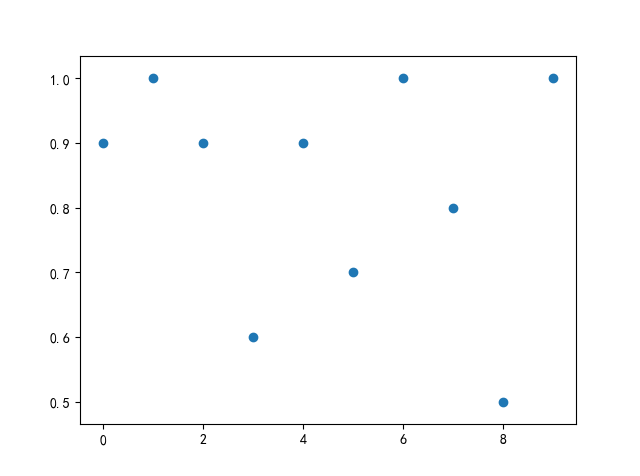
\includegraphics[width=5.5cm]{Acc1.png}
			\subcaption{流程图}
			\label{fig:sample-figure-a}
		\end{minipage}
		\begin{minipage}[t]{0.4\linewidth}
			\centering
			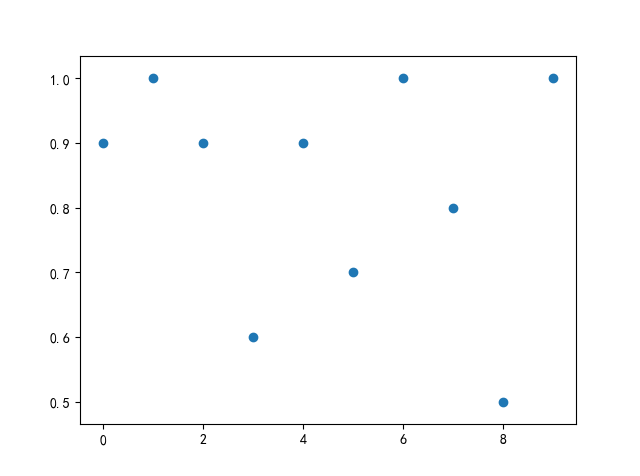
\includegraphics[width=5.5cm]{Acc1.png}
			\subcaption{流程图}
			\label{fig:sample-figure-b}
		\end{minipage}
	\quad
		\begin{minipage}[t]{0.4\linewidth}
			\centering
			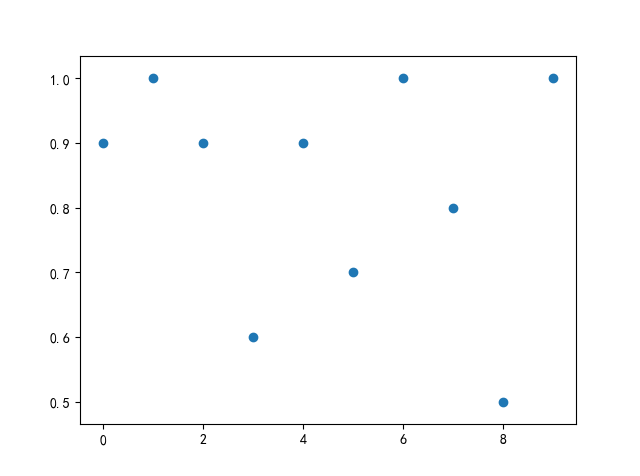
\includegraphics[width=5.5cm]{Acc1.png}
			\subcaption{流程图}
			\label{fig:sample-figure-c}
		\end{minipage}
		\begin{minipage}[t]{0.4\linewidth}
			\centering
			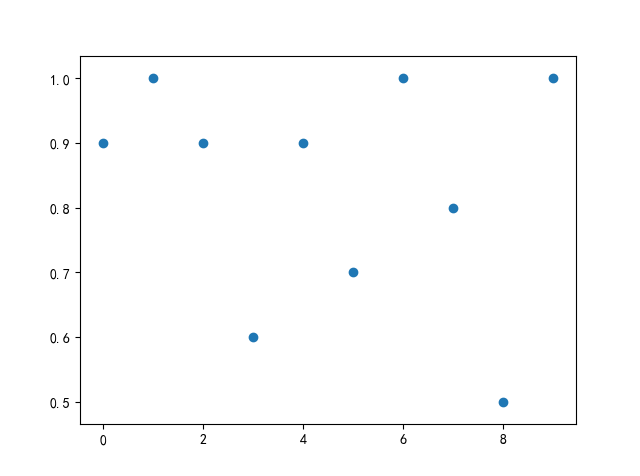
\includegraphics[width=5.5cm]{Acc1.png}
			\subcaption{流程图}
			\label{fig:sample-figure-d}
		\end{minipage}
	
	\centering
	\caption{设置子图}
\end{figure}



	\subsection{问题二分析}
	如果对葡萄酒进行\textbf{分级}
	
		\begin{figure}[H] %H为当前位置,!htb为忽略美学标准,htbp为浮动图形
			\centering %图片居中
			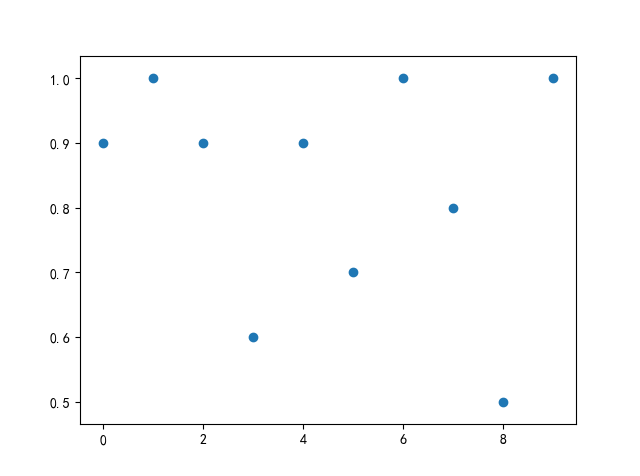
\includegraphics[width=0.7\textwidth]{Acc1.png} %插入图片,[]中设置图片大小,{}中是图片文件名
			%\caption{第五次作业} %最终文档中希望显示的图片标题
			%\label{Fig.main 2} %用于文内引用的标签
		\end{figure}
	
		

\section{问题一的求解}

这是一个求解

\section{问题二的求解}
这是一个求解

\subsection{一些可能用到}

无序列表是这样的:
\begin{itemize}
	\item 标准化处理
	\item 计算相关性
	\item 提取主成分,计算各主成分贡献率
\end{itemize}

有序列表是这样子的:
\begin{enumerate}
	\item 标准化处理
	\item 计算相关性
	\item 提取主成分,计算各主成分贡献率
\end{enumerate}

\begin{tcode}
	说不动会用到
	可以加上边框,感觉很秀
\end{tcode}

\par

\textbf{加粗字体}
\\
\textit{斜体 Italics}


\section{模型的评价与推广}
模型的优点是

%参考文献
\begin{thebibliography}{9}%宽度9
	\bibitem[1]{liuhaiyang2013latex}
	刘海洋.
	\newblock \LaTeX {}入门\allowbreak[J].
	\newblock 电子工业出版社, 北京, 2013.
	\bibitem[2]{mathematical-modeling}
	全国大学生数学建模竞赛论文格式规范 (2020 年 8 月 25 日修改).
	\bibitem[3]{mathematical-modeling}
	李航,统计学习方法,北京:清华大学出版社,2012.3。     
	\bibitem[4]{quanjing} Weisong Zhao,HMM隐马尔可夫模型详解,\url{https://blog.csdn.net/weixin_41923961/article/details/82750687},20(3),2021。(如何网页作为参考文献)
\end{thebibliography}

\newpage
%附录
\begin{appendices}
	
\section{matlab 源程序}
\begin{matlab}
	%支持中文
	kk=2;[mdd,ndd]=size(dd);
	while ~isempty(V)
	[tmpd,j]=min(W(i,V));tmpj=V(j);
	for k=2:ndd
	[tmp1,jj]=min(dd(1,k)+W(dd(2,k),V));
	tmp2=V(jj);tt(k-1,:)=[tmp1,tmp2,jj];
	end
	tmp=[tmpd,tmpj,j;tt];[tmp3,tmp4]=min(tmp(:,1));
	if tmp3==tmpd, ss(1:2,kk)=[i;tmp(tmp4,2)];
	else,tmp5=find(ss(:,tmp4)~=0);tmp6=length(tmp5);
	if dd(2,tmp4)==ss(tmp6,tmp4)
	ss(1:tmp6+1,kk)=[ss(tmp5,tmp4);tmp(tmp4,2)];
	else, ss(1:3,kk)=[i;dd(2,tmp4);tmp(tmp4,2)];
	end;end
	dd=[dd,[tmp3;tmp(tmp4,2)]];V(tmp(tmp4,3))=[];
	[mdd,ndd]=size(dd);kk=kk+1;
	end; S=ss; D=dd(1,:);
\end{matlab}

\begin{python}
	# 支持中文
	import numpy as np
	import pandas as pd
	import matplotlib.pyplot as plt
	import scipy as sci
\end{python}

\end{appendices}


\end{document}